\begin{figure*}[!t]
\centering
\begin{subfigure}{0.18\linewidth}

\includegraphics[width=\linewidth]{Images/mean.pdf}
\caption{$mean$}
\label{}
\end{subfigure}
\hspace{2mm}
\begin{subfigure}{0.18\linewidth}

\includegraphics[width=\linewidth]{Images/bvolumeT.pdf}
\caption{$bvolume_{T}$}
\label{}
\end{subfigure}
\hspace{2mm}
\begin{subfigure}{0.18\linewidth}

\includegraphics[width=\linewidth]{Images/distanceT.pdf}
\caption{$distance_{T}$}
\label{}
\end{subfigure}
\hspace{2mm}
\begin{subfigure}{0.18\linewidth}
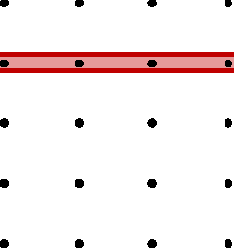
\includegraphics[width=\linewidth]{Images/zlsT.pdf}
\caption{$ZLS_{T}$}
\label{}
\end{subfigure}
\hspace{2mm}
\begin{subfigure}{0.18\linewidth}
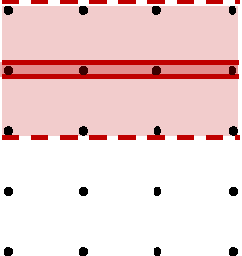
\includegraphics[width=\linewidth]{Images/zlsT_flsT.pdf}
\caption{$ZLS_{T}$ + $FLS_{T,1}$}
\label{}
\end{subfigure}
\begin{subfigure}{0.18\linewidth}

\includegraphics[width=\linewidth]{Images/sd.pdf}
\caption{$SD$}
\label{}
\end{subfigure}
\hspace{2mm}
\begin{subfigure}{0.18\linewidth}
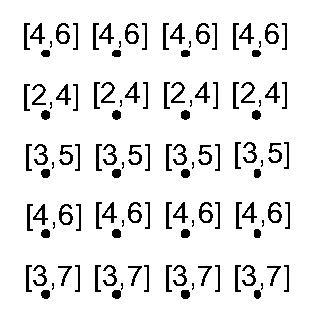
\includegraphics[width=\linewidth]{Images/boundsC.pdf}
\caption{$bounds_{C}$}
\label{}
\end{subfigure}
\hspace{2mm}
\begin{subfigure}{0.18\linewidth}
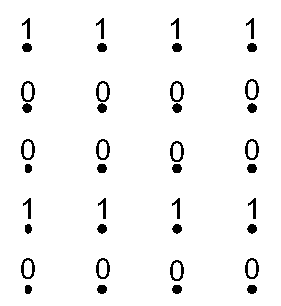
\includegraphics[width=\linewidth]{Images/bvolumeTC.pdf}
\caption{$bvolume_{T,C}$}
\label{}
\end{subfigure}
\hspace{2mm}
\begin{subfigure}{0.18\linewidth}
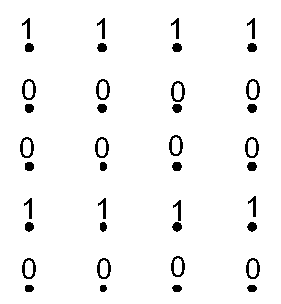
\includegraphics[width=\linewidth]{Images/distanceTC.pdf}
\caption{$distance_{T,C}$}
\label{}
\end{subfigure}
\hspace{2mm}
\begin{subfigure}{0.18\linewidth}
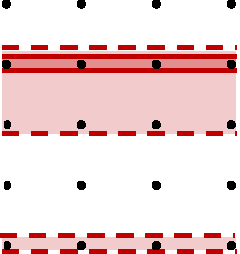
\includegraphics[width=\linewidth]{Images/zlsT_fclsTC.pdf}
\caption{$ZLS_{T}$ + $FCLS_{T,C}$}
\label{}
\end{subfigure}
\caption{Notional example}
\label{fig:example_sub}
\end{figure*}
